\documentclass{article}
\usepackage[utf8]{inputenc}
\usepackage{listings}
\usepackage{xcolor}
\usepackage{siunitx}
\usepackage{amsmath}
\usepackage{float}
\usepackage{graphicx}
\usepackage[italian]{babel}
\definecolor{keyword}{rgb}{0,0,1}
\definecolor{codegray}{rgb}{0.5,0.5,0.5}
\definecolor{string}{rgb}{0,0.7,0.2}
\definecolor{backcolour}{rgb}{1,1,1}

\lstdefinestyle{mystyle}{
    backgroundcolor=\color{backcolour},   
    commentstyle=\color{codegray},
    keywordstyle=\color{keyword},
    numberstyle=\tiny\color{codegray},
    stringstyle=\color{string},
    basicstyle=\ttfamily\footnotesize,
    breakatwhitespace=false,         
    breaklines=true,                 
    captionpos=b,                    
    keepspaces=true,                 
    numbers=left,                    
    numbersep=5pt,                  
    showspaces=false,                
    showstringspaces=false,
    showtabs=false,                  
    tabsize=2
}

\lstset{style=mystyle}

\renewcommand*\contentsname{Indice}

\title{Misura di temperatura con
sensore LM335 e
scheda Arduino Uno}
\author{Simone Aronica, Giovanni Bloise, \\
Gabriele Camisa, Giuseppe Casale}
\date{}

\begin{document}

\maketitle
\tableofcontents
\pagebreak

\section{Strumenti usati}
\begin{itemize}
    \item Arduino Uno, utilizzato come ADC 
    \begin{itemize}
        \item risoluzione di 10 bit 
        \item alimentazione tramite porta USB 2.0 ($V_{\text{CC}} = 5 \pm \SI{0.25}{\volt}$).
        \item tensione di riferimento interna all'ADC $V_{\text{int}} = 1.1 \pm \SI{0.1}{\volt}$.
    \end{itemize}
    \item Sensore LM335, trasduttore di temperatura 
    \begin{itemize}
        \item $V_{\text{out}} = \SI{10}{\milli\volt} \cdot T$
        \item campo di temperatura: $(-40\div100)\SI{}{\celsius}$
        \item uscita riferita allo zero assoluto: $V_{\text{out}} = \SI{0}{\volt}\ @ \SI{-273,15}{\celsius}$
        \item sensibilità nominale $S = \SI{10}{\milli\volt\per\kelvin}$
        \item incertezza strumentale a temperatura ambiente (modello deterministico): $\delta T = \SI{2}{\celsius}$
        \item resistenza termica: $\SI{165}{\celsius\per\watt}$
    \end{itemize}
    \item Multimetro HP 34401A
\end{itemize}

\section{Sintesi dell'esperienza}
L'esperienza consiste nella misurazione della temperatura ambientale all'interno del laboratorio mediante l'impiego di una scheda Arduino Uno a cui è stato collegato un sensore National Semiconductors LM335. Nei seguenti paragrafi saranno descritte le due configurazioni utilizzate e verrà valutata l'incertezza attesa.

\section{Prima configurazione}
Il sensore è stato collegato ad alimentazione tramite USB 2.0 ($5 \pm \SI{0.25}{\volt}$), ponendo attenzione ad evitare un effetto di autoriscaldamento che andasse a falsare i valori ottenuti, ovvero a mantenere la corrente di funzionamento nel range appropriato ($\SI{0.4}{\milli\ampere}<i<\SI{5}{\milli\ampere}$, reperibile dal datasheet). 
Ipotizzando che la temperatura ambientale sia tra $\SI{5}{\celsius}$ e $\SI{50}{\celsius}$ (tra $\SI{278}{\kelvin}$ e $\SI{323}{\kelvin}$) e considerando la sensibilità nominale di $\SI{10}{\milli\volt\per\kelvin}$, è stata quindi scelta una resistenza appropriata da inserire in serie all'alimentazione. Dalla risoluzione delle disequazioni
\begin{align*}
    I_{D,\min}=\frac{V_s-V_{\text{out}, \max}}{R_1} > \SI{0.4}{\milli\ampere}\\
    I_{D,\max}=\frac{V_s-V_{\text{out}, \min}}{R_1} < \SI{5}{\milli\ampere}
\end{align*}
una resistenza di $\SI{1}{\kilo\Omega}$ risulta accettabile.
\begin{figure}[H]
    \centering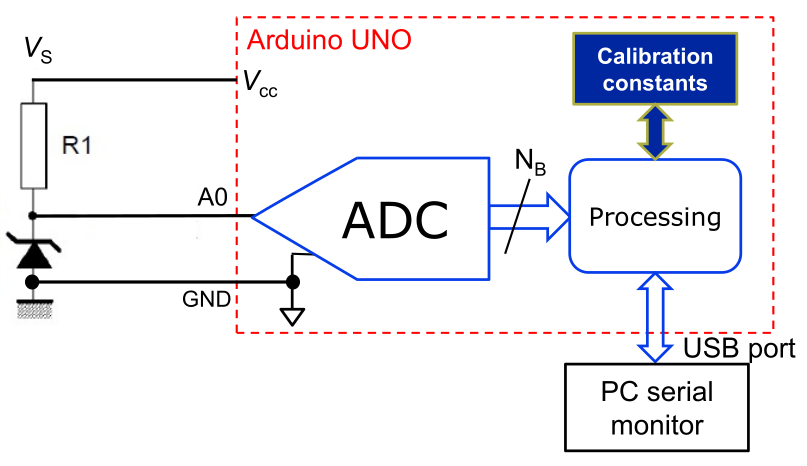
\includegraphics[width=200px]{img/circuito_1.png}
    \caption{Schema circuitale della prima configurazione}
\end{figure}

\subsection{Firmware}
La funzione di taratura
\begin{equation*}
    T=D_{\text{out}}\cdot\frac{V_{\text{FR}}}{2^{\text{N}_\text{B}}}\cdot\frac{1}{S}
\end{equation*}
è stata implementata, insieme alla visualizzazione delle misure di temperatura in Celsius e Kelvin, nel seguente codice sorgente:
\begin{lstlisting}[language=C]
const int pin = A3;
const int Vcc = 5; // alimentazione USB 2.0
const int Nbit = 10; // bit ADC
const int S = 0.01; // da: Vout = 10mV * T_K

void setup() {
  pinMode(A3, INPUT);
  Serial.begin(9600); // baud rate
}

void loop() {
  int Dout = analogRead(pin); 
  float T_K = Dout * Vcc / pow(2, Nbit) * 1/S; 

  Serial.print("Valore sensore: ");
  Serial.println(Dout);
  Serial.print("Temperatura in Kelvin: ");
  Serial.println(T_K);
  Serial.print("Temperatura in Celsius: ");
  Serial.print(T_K - 273.15);
  Serial.println("######");

  delay(1000);
}
\end{lstlisting}
Dalla misurazione si ricava un valore di $\SI{26.85}{\celsius}$ e $D_{\text{out}, \max}=800$.
\subsection{Valutazione dell'incertezza}
Si è proceduto a valutare l'incertezza della misurazione tramite il modello deterministico:
\begin{equation*}
    \begin{split}
        \delta T&=\left|\frac{\partial T}{\partial D_{\text{out}}}\right|\delta D_{\text{out}}+\left|\frac{\partial T}{\partial V_{\text{FR}}}\right|\delta V_{\text{FR}}+\left|\frac{\partial T}{\partial S}\right|\delta S=\\
        &=\frac{V_{\text{FR}}}{S\cdot2^{\text{N}_\text{B}}}\delta D_{\text{out}}+\frac{D_{\text{out}}}{S\cdot2^{\text{N}_\text{B}}}\delta V_{\text{FR}}+\delta T^{\text{sensor}}
    \end{split}
\end{equation*}
da cui, sostituendo i valori effettivi:
\begin{equation*}
    \begin{split}    
        \delta T&=\frac{\SI{5}\volt}{\SI{10}{\milli\volt\per\kelvin}\cdot2^{10}}\cdot 2+\frac{800}{\SI{10}{\milli\volt\per\kelvin}\cdot 2^{10}}\cdot\SI{0.25}{\volt}+\SI{2}{\kelvin}\approx\\&\approx \SI{0.98}{\kelvin}+\SI{19.53}{\kelvin}+\SI{2}{\kelvin}=\SI{22.51}{\kelvin}
    \end{split}    
\end{equation*}
Correlata dell'incertezza, risulta $T = \SI{26.85}{\celsius}, 84\%$.
\section{Seconda configurazione}
È facile notare come, nella configurazione precedente, il massimo contributo di incertezza sia dato dal termine $\frac{D_{\text{out}}}{S\cdot2^{\text{N}_\text{B}}}\delta V_{\text{FR}}\approx\SI{19.53}{\kelvin}$. Per ridurlo, è
possibile sostituire la tensione di riferimento del sistema (fino ad ora la stessa tensione di alimentazione, su cui si ha un'incertezza relativa del $5\%$) con una tensione di cui si conosce un valore più accurato. Un esempio
è il riferimento interno all'ADC della scheda Arduino Uno $(V_{\text{int}}=1.1\pm\SI{0.1}{\volt})$, che è stato utilizzato nella seconda fase dell'esperienza.
\subsection{Modifiche al circuito di condizionamento}
Il cambio di riferimento rende necessaria una modifica alla struttura del circuito di condizionamento, al fine di indurre un'attenuazione del segnale di uscita del sensore. L'attenuazione è stata realizzata tramite l'inserimento di due resistenze, 
$R_2$ ed $R_3$, posizionate in modo tale da poter prelevare dai capi di $R_3$ una partizione della tensione $V_\text{out}$ di partenza.
\begin{figure}[H]
    \centering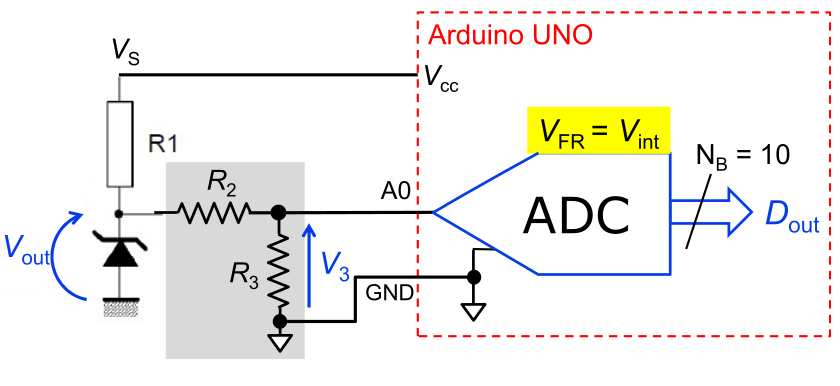
\includegraphics[width=200px]{img/circuito_2.png}
    \caption{Schema circuitale della seconda configurazione}
\end{figure}
I valori di tali resistenze sono stati determinati in modo da ottenere una attenuazione $\ge 3$; in particolare sono state scelte 
$R_2 = \SI{68}{\kilo\Omega}$ e $R_3=\SI{33}{\kilo\Omega}$. Dalla misurazione delle stesse con il multimetro digitale sono emerse le misure $R_2=\left(68610.00\pm7.86\right)\SI{}{\Omega}$ e $R_3=\left(32570.00\pm4.26\right)\SI{}{\Omega}$.
Il valore ottenuto dalla misurazione della temperatura ambientale con questa seconda configurazione si è attestato su $\SI{18.18}{\celsius}$, con $D_{\text{out}, \max} = 903$.
\subsection{Modifiche al firmware}
Il cambio della tensione di riferimento si realizza nel firmware, tramite l'aggiunta della direttiva

\lstdefinestyle{mystyle}{
    numberstyle=\tiny\color{backcolour},
}
\lstset{style=mystyle}

\begin{lstlisting}[language=C]
    analogReference(INTERNAL); 
\end{lstlisting}    
all'interno della funzione \texttt{setup}.
In seguito alle modifiche al circuito di condizionamento, la funzione di taratura è da ridefinire come:
\begin{equation*}
    T=D_{\text{out}}\cdot\frac{V_{\text{int}}}{2^{\text{N}_\text{B}}}\cdot\frac{1}{S}\cdot\left(1+\frac{R_2}{R_3}\right)
\end{equation*}
La modifica si riflette nel sorgente nel modificare la definizione di \texttt{T\_K} di riga 13.
\begin{lstlisting}[language=C]
    float T_K = Dout * Vcc / pow(2, Nbit) * 1/S * (1 + R2/R3);
\end{lstlisting}    
\subsection{Valutazione dell'incertezza}
\begin{equation*}
    \begin{split}    
        \delta T&=\left|\frac{\partial T}{\partial D_{\text{out}}}\right|\delta D_{\text{out}}+\left|\frac{\partial T}{\partial V_{\text{int}}}\right|\delta V_{\text{int}}+\left|\frac{\partial T}{\partial S}\right|\delta S+\left|\frac{\partial T}{\partial R_2}\right|\delta R_2+\left|\frac{\partial T}{\partial R_3}\right|\delta R_3 =\\
        &=\frac{V_{\text{int}}}{S\cdot2^{\text{N}_\text{B}}}\delta D_{\text{out}}+\frac{D_{\text{out}}}{S\cdot2^{\text{N}_\text{B}}}\delta V_{\text{int}}+\delta T^{\text{sensor}}+\\
        &+\frac{D_{\text{out}}V_{\text{int}}}{S\cdot2^{\text{N}_\text{B}}\cdot R_3}\delta R_2-\frac{D_{\text{out}}V_{\text{int}}R_2}{S\cdot2^{\text{N}_\text{B}}\cdot {\left(R_3\right)}^2}\delta R_3
    \end{split}    
\end{equation*}
da cui si ricava:
\begin{equation*}
    \begin{split}
        \delta T&=\frac{\SI{1.1}\volt}{\SI{10}{\milli\volt\per\kelvin}\cdot2^{10}}\cdot 2+\frac{903}{\SI{10}{\milli\volt\per\kelvin}\cdot 2^{10}}\cdot\SI{0.1}{\volt}+\SI{2}{\kelvin}+\\
        &+\frac{903\cdot\SI{1.1}{\volt}}{\SI{10}{\milli\volt\per\kelvin}\cdot 2^{10}\cdot \SI{32570}{\Omega}}\cdot\SI{7.86}{\Omega}+\\
        &- \frac{903\cdot\SI{1.1}{\volt}\cdot\SI{68610}{\Omega}}{\SI{10}{\milli\volt\per\kelvin}\cdot 2^{10}\cdot{\left(\SI{32570}{\Omega}\right)}^2}\cdot\SI{4.26}{\Omega}=\\
        &=\SI{11.03}{\kelvin}
    \end{split}
\end{equation*}
per cui dalla misura della temperatura ambientale con la seconda configurazione risulta infine: $T = \SI{18.18}{\celsius}, 60\%$.
\section{Conclusioni}
Si è sperimentata la realizzazione di un circuito di condizionamento tramite Arduino Uno in due diverse configurazioni e valutata l'incertezza sulla misurazione che ne è derivata. In particolare, si è notato come la seconda configurazione abbia portato ad un significativo miglioramento sull'incertezza della misura dichiarata. 

L'esperienza ha quindi dimostrato l'importanza del progetto preliminare del circuito di condizionamento sul risultato delle operazioni di misura
e ha costituito un esempio di quali siano i criteri da ricercare in tale circuito (in questo caso, un contributo di incertezza minimo sulla tensione utilizzata come riferimento).
Le misurazioni derivate dalle due configurazioni sono tra loro compatibili e a loro volta confrontabili con una stima personale delle reali condizioni di temperatura dell'ambiente del laboratorio. 
\end{document}
